\documentclass[main.tex]{subfiles}

\begin{document}

\renewcommand{\labelitemi}{\ding{226}}
\renewcommand{\labelitemii}{\ding{227}}

\newcommand{\sfgdx}{192}
\newcommand{\sfgdy}{184}
\newcommand{\sfgdz}{56}

\chapter{Super FGD}
\label{ch:up:sfgd}
In the ND280, the Fine-Grained Detectors (FGD)~\cite{Amaudruz2012} serves as neutrino targets. They are made from scintillator bars oriented in the perpendicular directions w.r.t the neutrino beam. Such a structure provides an excellent performance in the reconstruction of the forward-going tracks. \autoref{fig:up:sfgd:fgd} shows the scheme of the current FGD modules. From the figure one can see that an acceptance for tracks at a high angle is limited. The whole track may be contained in a one scintillator bar and the accurate measurement will not be possible. One of the main goals of the ND280 upgrade is to study tracks at a high angle, thus a target with a new concept is required.

\begin{figure}[!ht]
	\centering
	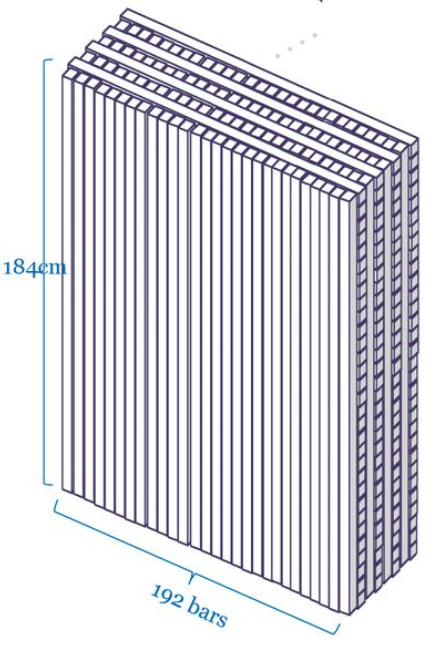
\includegraphics[width=0.3\linewidth]{FGD}
	\caption{The scheme of the exciting Fine-Grained Detector modules. Such a structure has a limited acceptance for the tracks at a high angle w.r.t. the beam.}
	\label{fig:up:sfgd:fgd}
\end{figure}

\section{Conceptual design}
A new target is going to be build with the optically isolated scintillator cubes. Each cube will have three holes in x, y, and z directions. The signal readout is organized with wavelength shifting fibers (WLS) that will transfer light to the Multi--Pixel Photo Counters (MPPC). With such a concept, the events will be reconstructed in three projections that can be further merged into a 3D image. The scheme of the concept is shown in \autoref{fig:up:sfgd:gen}.

\begin{figure}[!ht]
	\centering
	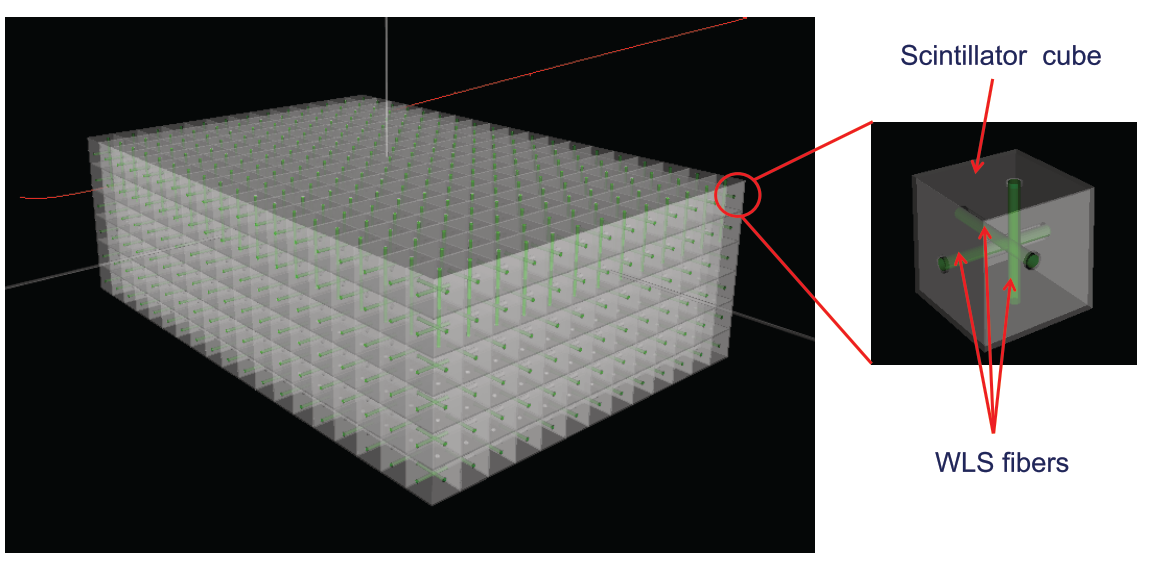
\includegraphics[width=0.8\linewidth]{sfgd_gen}
	\caption{The schematic concept of the SuperFGD detector made with scintillator cubes. Wavelength shifting fibers are used for the signal readout. The size of each cube is 1$\times$1$\times$1 $\text{cm}^3$.}
	\label{fig:up:sfgd:gen}
\end{figure}

The detector dimensions are \sfgdx$\times$\sfgdy$\times$\sfgdz  cubes 1$\times$1$\times$1 $\text{cm}^3$ each. The total number of cubes and channels will be 1885632 and 54224 respectively. The details about the cubes characteristics are provided in \autoref{sec:up:sfgd:cube}. The MPPCs will be placed on the upstream, top, left and right side of the detector. The front--end electronics, including the digitizers is going to be built on site. The digitized signal will be transported through the optical fiber outside the magnet to the ND280 data acquisition system. More details about the electronics can be found in \autoref{sec:up:sfgd:ele}.

\subsection{Scintillator cubes}
\label{sec:up:sfgd:cube}
The scintillator cubes are made from polystyrene doped with 1.5\% of paraterphenyl (PTP) and 0.01\% of POPOP. The cubes production is done with the injection molding with the press-form. Ten cubes could be produced at one act of molding that speeds up the mass production of the detector. The molding technology also increases the cube size accuracy comparing to the extrusion technology that is usually used for the scintillator detectors production. Cube dimensions accuracy is critical as we are going to assemble the detector from nearly 2 million of cubes. Size fluctuation are required to be minimal to prevent cube's holes misalignment because of the position fluctuations.

\begin{figure}[!ht]
	\centering
	\begin{minipage}{0.49\linewidth}
		\centering
		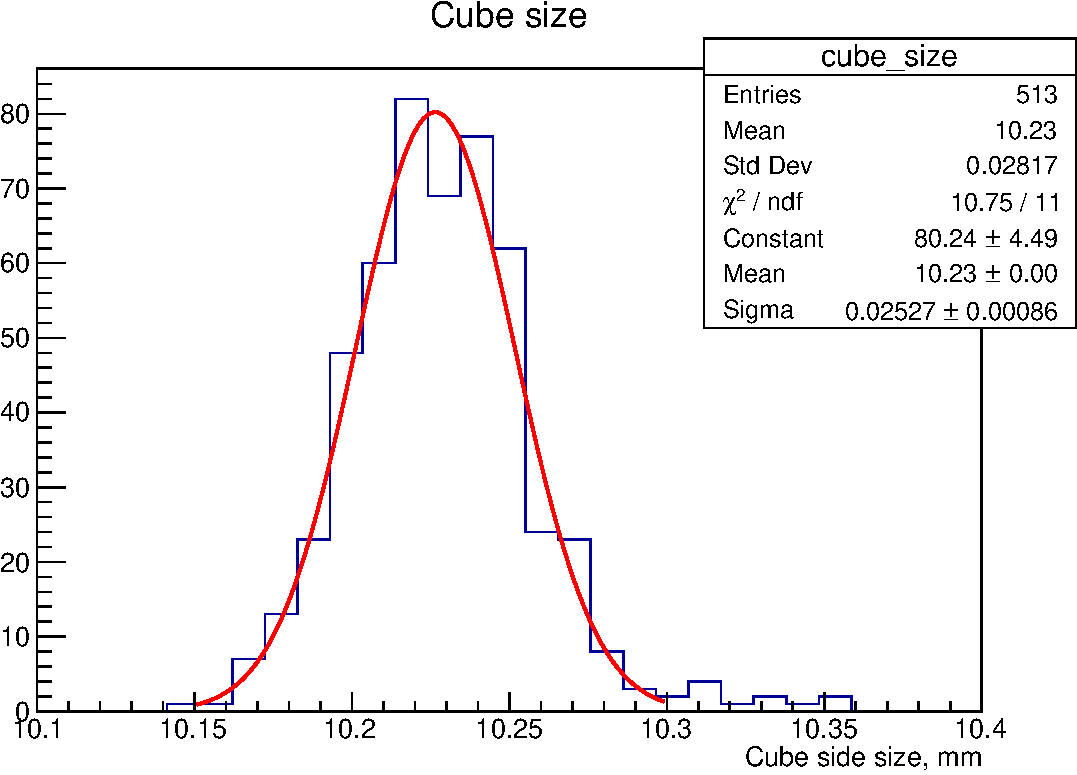
\includegraphics[width=\linewidth]{cube_size}
		\caption{The accuracy of the cube dimensions after the etching with a reflector. The results of 513 measurements are fit and demonstrates 25 $\mu$m accuracy.}
		\label{fig:up:sfgd:cube_s}
	\end{minipage}
	\begin{minipage}{0.49\linewidth}
		\centering
		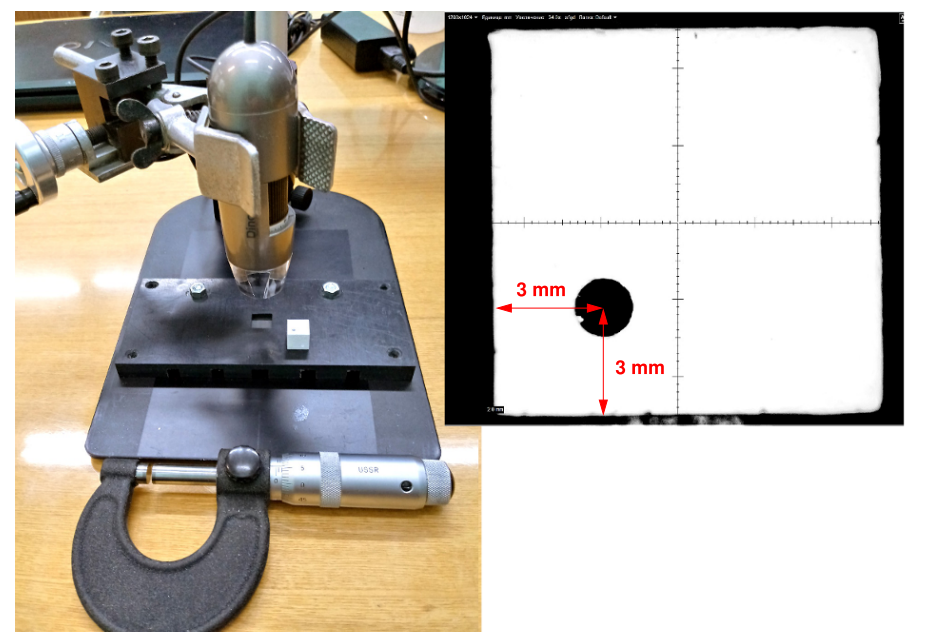
\includegraphics[width=\linewidth]{hole_measurements}
		\caption{The digital microscope used for the measurements of the hole position}
		\label{fig:up:sfgd:hole_pos}
	\end{minipage}
\end{figure}

After the molding, the cubes are covered by a chemical diffuse reflector by etching the scintillator surface in a chemical agent. The fluctuations of the cube size were measured after the etching procedure. The results are shown in \autoref{fig:up:sfgd:cube_s} and demonstrates the Gaussian behavior with 25 $\mu$m accuracy. Afterwards three holes with a 1.5 mm diameter are drilled. The positions of the holes are also precisely controlled with the digital microscope (\autoref{fig:up:sfgd:hole_pos}). Variations at the level of 80 $\mu$m were observed. Since the fiber diameter is 1 mm while the hole size is 1.5 mm, this is not supposed to bring a problem during the assembly. The cube size fluctuations remains the main challenge for the detector construction.

\subsection{Assembly}
\label{sec:up:sfgd:ass}
The assembly of the detector needs to be designed carefully. The setup requires aligning all the cubes at their position in three dimensions and easy inserting the WLS fibers. With the given number of 2 million cubes and with measured uncertainties on cube size and hole positions, this is a challenging task.

\subsubsection{Loose structure}
We considered creating a loose structure of cubes self--aligned with fishing lines. The key idea is to fully assemble the detector with 1.2 mm fishing lines instead of the 1 mm WLS. Cubes positions are fixed only with these lines without the precise control over the position of each cube. Then the fishing line will be replaced one by one with the fibers. As WLS fiber diameter is smaller comparing to the fishing line it should be easy to perform such a replacement. During the whole replacement procedure cubes are aligned with lines and fibers. Such a technique will also protect the fibers that are quite expensive and fragile. They are going to be inserted only at the final stage of detector construction.

Detector assembly starts from the string construction (\autoref{fig:up:sfgd:string} (a)). A line of \sfgdx cubes is assembled on the fishing line. The set of \sfgdy strings is joint line by line to the plane \sfgdx$\times$\sfgdy (\autoref{fig:up:sfgd:string} (b)). Planes are put on top of the each other to form a full detector (\autoref{fig:up:sfgd:string} (c)). The planes will be aligned so that the fishing lines will be inserted in the vertical holes as well. The alignment along the 3rd axis is the most difficult part of the assembly. The loose structure allows to solve this problem with the small cube displacements during the insertion the fishing line in 3rd axis.

\begin{figure}[!ht]
	\centering
  \begin{minipage}{0.33\linewidth}
    \centering
    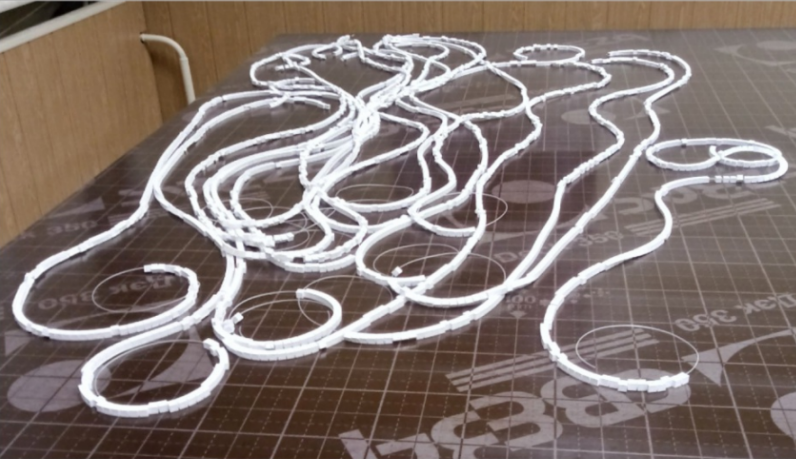
\includegraphics[width=\linewidth]{sfgd_FL_1} \\ (a)
  \end{minipage}
  \begin{minipage}{0.33\linewidth}
    \centering
    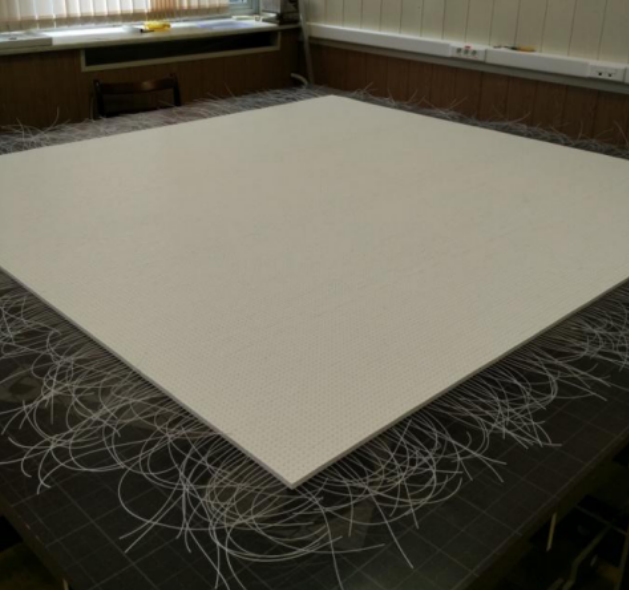
\includegraphics[width=\linewidth]{sfgd_FL_2} \\ (b)
  \end{minipage}
  \begin{minipage}{0.33\linewidth}
    \centering
    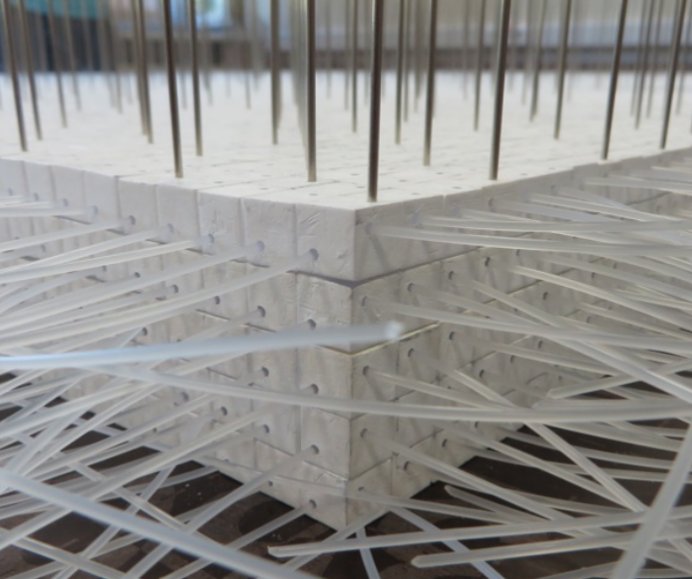
\includegraphics[width=\linewidth]{sfgd_FL_3} \\ (c)
  \end{minipage}
  \caption{The assembly technology of the SFGD detector with the fishing lines. The technology starts from the string assembly (a) that are further merged into the planes (b). Finally, the planes are put on top of the each other and the vertical holes are aligned with steel needles(c).}
  \label{fig:up:sfgd:string}
\end{figure}

Several tests of the assembly were performed. The first one includes a 2 m long prototype with the transversal dimensions 6$\times$6 cubes. This prototype was aimed to test the robustness of the assembly strategy, the possibility of the lines replacement with WLS, the length fluctuations of the 2 m long setup. The photos of the prototype are presented in \autoref{fig:up:sfgd:long}. With such a test it was proved that we can construct the detector with the proposed method. The tests were performed with and without a 50 kg payload on the top cover of the detector. In both cases the fishing lines can be easily replaced by fibers. The friction of the fishing line with the 200 cubes is small and the line can be easily removed. There is no strong friction during the fiber insertion as well. The length of the prototype was in agreement with the expectations within the 1 mm accuracy.

\begin{figure}[!ht]
	\centering
  \begin{minipage}{0.49\linewidth}
    \centering
    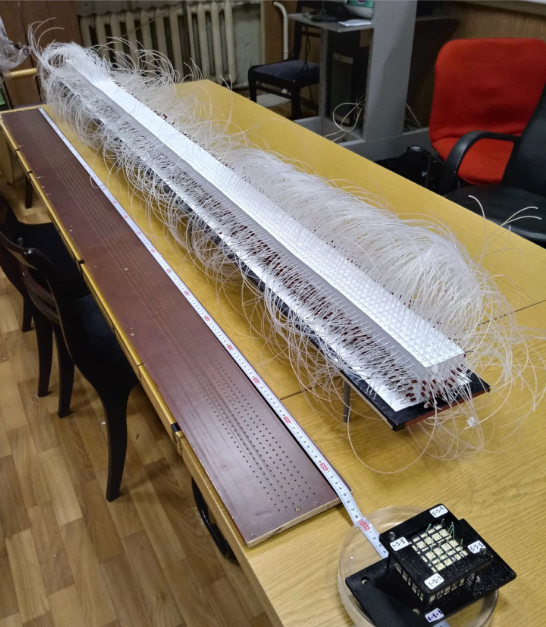
\includegraphics[width=0.5\linewidth]{sfgd_len_1} \\ (a)
  \end{minipage}
  \begin{minipage}{0.49\linewidth}
    \centering
    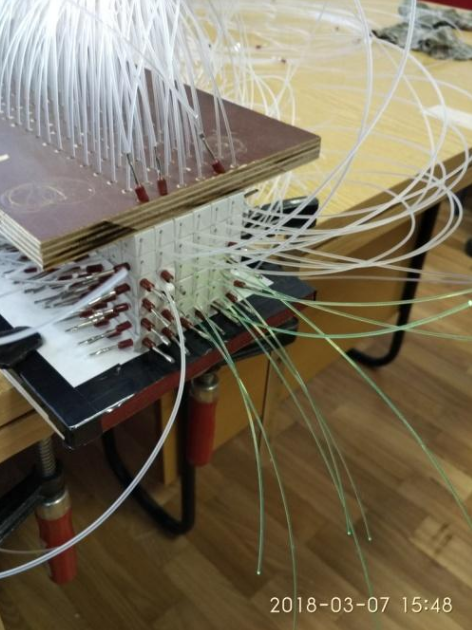
\includegraphics[width=0.5\linewidth]{sfgd_len_2} \\ (b)
  \end{minipage}
  \caption{Photos of the detector prototype built with 200$\times$6$\times$6 cubes. Cubes assembled with the fishing line (a) and after the replacement of several lines with WLS fibers (b).}
  \label{fig:up:sfgd:long}
\end{figure}

Two prototypes were build for the detector tests with the beam of charged particles. This prototypes served also as an assembly technology tests. The first one was quite small 5$\times$5$\times$5 cubes. The second one was slightly larger and contained 48$\times$24$\times$8 cubes. Details about prototypes construction and beamtest results will be overviewed in \autoref{sec:up:sfgd:beam}.

After the successful beamtests the tall ``tower'' was build with 15$\times$56$\times$192 cubes. The main purpose of this prototype was to test the possibility of the fishing lines replacement with the WLS fibers in a toll and long structure of cubes. It was confirmed that such a detector could be build with fishing lines and they could be replaces with the fibers afterwards. The photo of the prototype is shown in \autoref{fig:up:sfgd:toll}. In addition, the test of the SuperFGD box strength and deformations was performed with this prototype. The details about the detector box will be provided in the next section.

\begin{figure}[!ht]
	\centering
	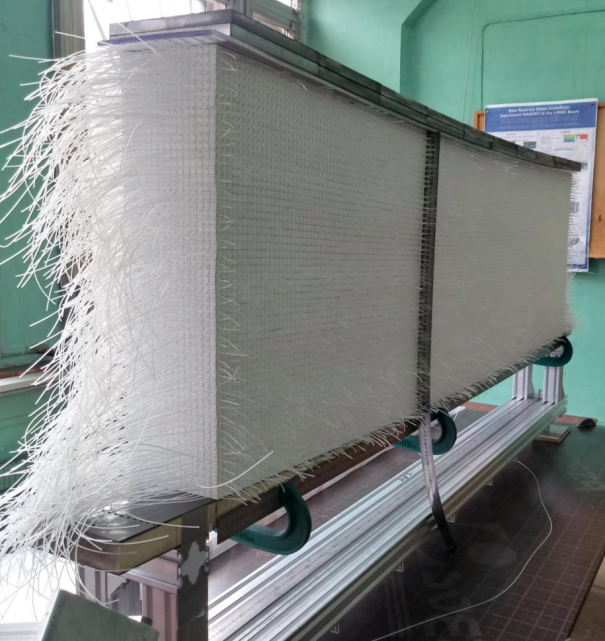
\includegraphics[width=0.3\linewidth]{sfgd_toll}
	\caption{The tall prototype of the SuperFGD detector made with 15$\times$56$\times$192 cubes.}
	\label{fig:up:sfgd:toll}
\end{figure}

\subsubsection{SuperFGD mechanics}
Mechanical structure of the scintillator target should provide a robust detector fixation to minimize the detector deformation due to load. The loose structure of cubes is a subject of deformation, while the WLS fibers are fragile and can be broken with the cube offset. At the same time the dead space between the target and HA--TPC is desired to be as small as possible to gain the precision of charged particles tracking. The mechanical structure should provide the optical interface to readout all the channels and host the calibration system.

To meet these requirements, the walls of the box are made from 16 mm AIRAX core laminated with 2 mm CF skins and are screwed together. The box is drilled with 3 mm holes providing the exit for every WLS fiber. Three of six walls carry signal readout system. The MPPCs are soldered on printed circuit boards (PCB) that are screwed on the CF box. On the readout sides the fibers are equipped with optical connectors to provide reliable light transfer to MPPC. The CAD of the optical interface and readout system is shown in \autoref{fig:up:sfgd:optics}. The other fibers endings are covered with the plastic coverage screwed to the box. This coverage shades the fibers from external light and also hosts the calibration system.

\begin{figure}[!ht]
	\centering
	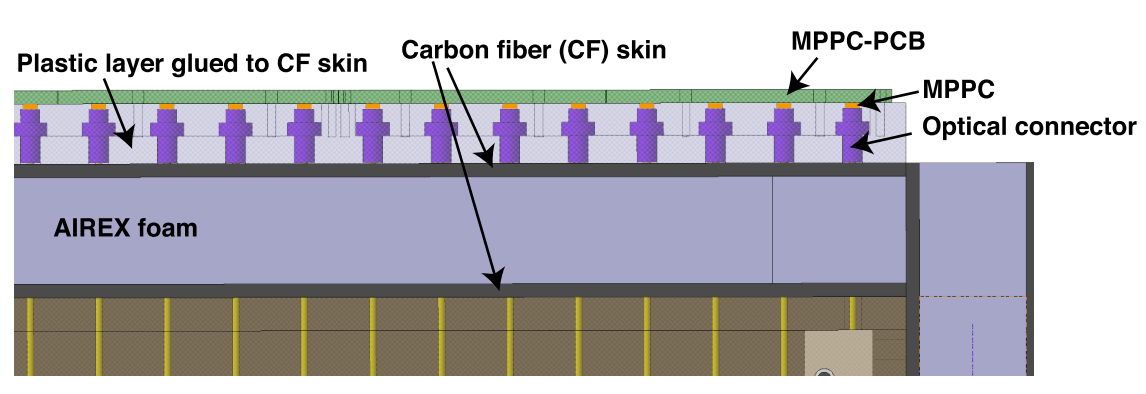
\includegraphics[width=0.7\linewidth]{optics}
	\caption{The optical interface of the SuperFGD detector}
	\label{fig:up:sfgd:optics}
\end{figure}

The deformation of the mechanical support structure was tested with the long and tall SuperFGD prototype (15$\times$56$\times$192 cubes). The measured sagitta was at the level of 20 mm. This value is close to the distance between the detectors but still meets the requirements and makes possible the detector assembly.

The calibration system is required to measure the MPPC gain, i.e. associate the output MPPC channel with the number of detected photoelectrons. In the current FGD we use MPPC with a high noise rate that allows to perform a calibration with the noise only. In the SuperFGD new low-noise MPPC will be used. It will make the signal more clean, but will require the external light injection system for calibration. The Light Guide Plane (LGP) is used for this purpose. On the non-readout side of the fibers the plastic plate is glued to the SuperFGD box. The light will be injected with LEDs at the plate border. The notches in the plate are made opposite to the fibers ends to scatter some light into the fibers (\autoref{fig:up:sfgd:calib}). With such a system the gain of each channel can be monitored continuously. It is especially important at the assembly stage to check all the MPPCs and fibers operate normally.

\begin{figure}[!ht]
	\centering
	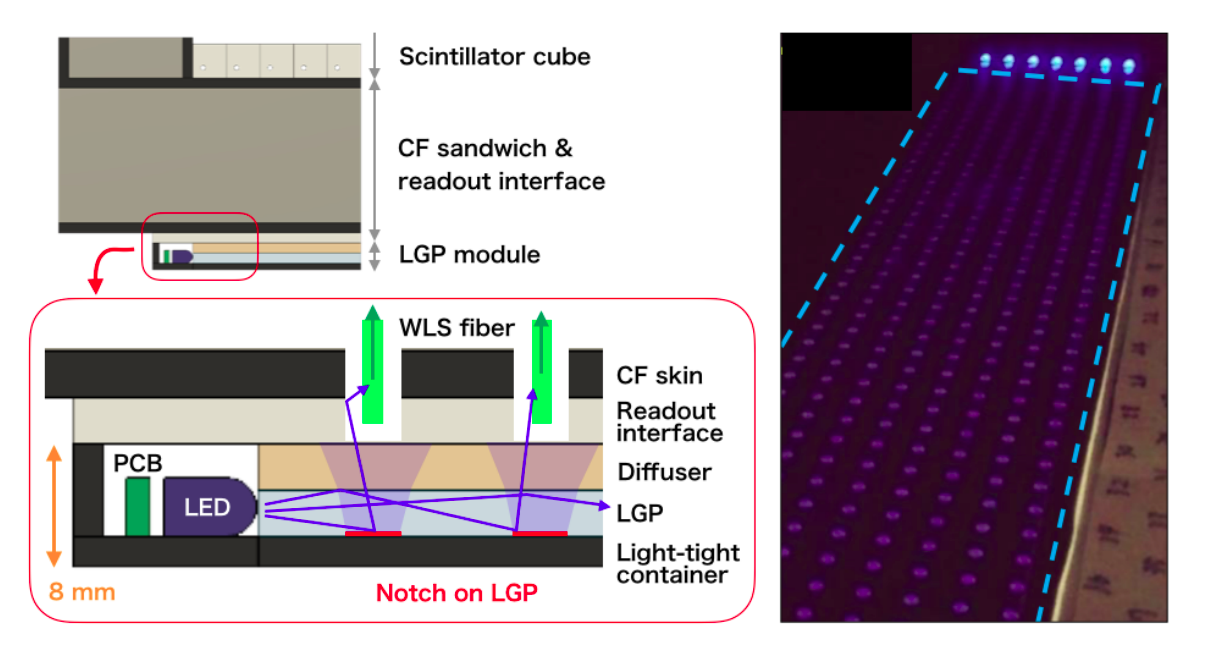
\includegraphics[width=0.7\linewidth]{calibration}
	\caption{SuperFGD calibration system with Light Guide Plane (left) and a LGP prototype (right).}
	\label{fig:up:sfgd:calib}
\end{figure}

\section{Electronics}
\label{sec:up:sfgd:ele}
SuperFGD electronics should measure the signal amplitude at every channel at every bunch of the neutrino beam. In T2K 8 bunches are separated with 600 ns and forms a spill that comes every 2 seconds. The readout system should be compatible with this regime. High dynamic range and precise timing are required for the precise physics measurement. Nucleons produced in the neutrino interactions are mostly low-energetic and stops shortly with large energy deposition. Since accurate spectroscopy of the nucleons are required for the neutrino interactions measurements, high dynamic range is essential. Time measurement is important for dividing particles directed to/from the target. The ToF system around the SFGD and HA--TPCs measures time with 100 ns accuracy. At our energies the SFGD time resolution at the level of 1 ns is enough for the reliable estimation of the track direction.

The electronics system based of the CITIROC chips (Cherenkov Imaging Telescope Integrated Read Out Chip) was chosen as a baseline option. These chips are used in BabyMIND~\cite{Blondel2015b} experiment in the T2K near detector complex. Thus these chips were designed to operate with scintillator detector at the same neutrino beam and therefore are compatible with the beam timing. CITIROC electronics suits the requirements of the dynamic range and time resolution. It stores signal in both log--gain and high--gain regime simultaneously and thus provides accurate amplitude measurements for both low and high light yield. At the moment, the bottle--neck of the dynamic range is a number of pixels in the MPPC. But our S13360-1325PE MPPCs carry 2668 and this is more then enough for the precise measurements. The sampling rate of the CITIROC ship is 400 MHz (2.5 ns). That brings us below 1 ns time resolution per channel.

Front--End Boards (FEB) are mounted in towers on both sides of SGFD inside the magnet. PCB are connected with the FEB with the coaxial cables. Such a scheme minimize the dead material between the SFGD and HA--TPC. FEB provides signal amplification, digitization, and zero--suppression. The optical cable transmit the data outside the magnet to the ND280 global DAQ system. This connection serves for the time synchronization as well.

\section{Simulations}
To estimate the behavior and main physical characteristics of the future detector I performed a bunch of simulations.

\subsection{Expected light yield}
On of the goals was to estimate the light yield of the detector with different particle types. As we are using 2 m long fibers the light attenuation is critical. The decision about fiber far end coverage should be taken. It could be mirrored and provide more light, but degrade the time resolution.

TODO

\subsection{Michell electron tagging}
The next quick check is understanding of the detector efficiency for Michell electron tagging. Michell electrons are produced in the muon decay $\mu\to e+\overline{\nu}_e+\nu_\mu$. They are quite useful for the identification of the muon from the neutrino interactions, thus we are interested in our detector efficiency.

TODO

\subsection{Pileups}

TODO




\section{Beamtest}
\label{sec:up:sfgd:beam}
Several beamtests were performed to evaluate the detector performance and characteristics.

\subsection{First CERN beamtest}
\label{sec:up:sfgd:beam1}
The first ever test was done with the small 5$\times$5$\times$5 cubes prototype. The main goals of the test were first measurement of the light yield and time resolution with the beam of charged particles. A Photo of the first prototype is shown in \autoref{fig:up:sfgd:1st}.

\begin{figure}[!ht]
	\centering
	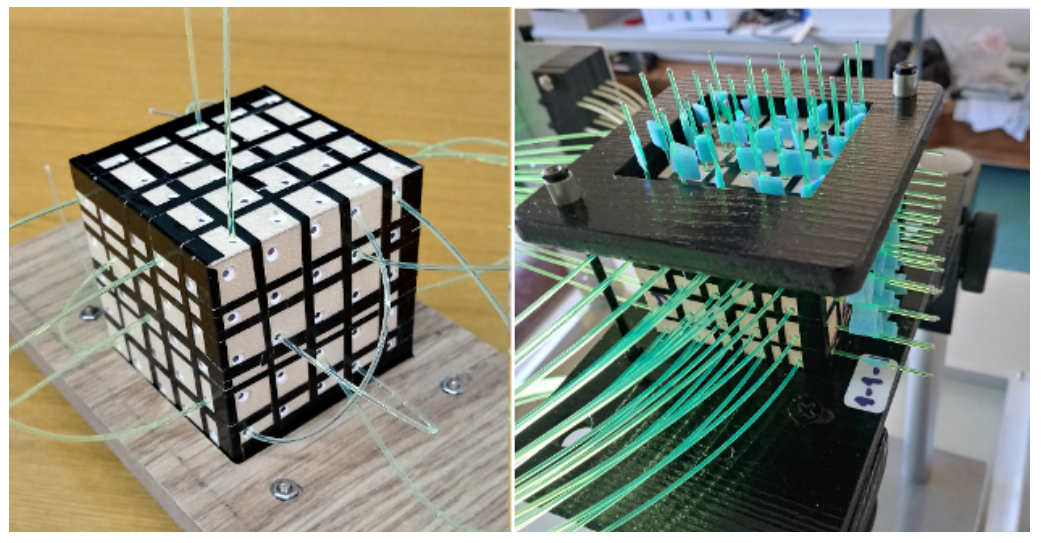
\includegraphics[width=0.5\linewidth]{fst_photo}
	\caption{The first 5$\times$5$\times$5 cubes prototype of the SuperFGS detector. The assembly stage (left) and a complete prototype with inserted WLS readout fibers (right).}
	\label{fig:up:sfgd:1st}
\end{figure}

The beamtest was performed at the T10 area of the CERN Proton Synchrotron (PS). The 6 GeV/c beam consisted mostly from positron and protons. Two scintillator bars were installed in 26 cm before and after the prototype and used as a trigger and reference measurements for the time resolution studies.

The light was readout in the two directions perpendicular to the beam. The distribution of the sum of the light yield from both channels is shown in \autoref{fig:up:sfgd:1st_res} (a). So we observed in average 80 photo electrons from one cube that is enough for the particle tracking and accurate time measurements. The time resolution was measured with respect to the time measurements in both trigger bars. A 5 GHz digitizer was used for sampling the data from the detector. Combing the measurements with two fibers in the same cube we reached a time resolution at the level of 650 ps (\autoref{fig:up:sfgd:1st_res} b). This result is beyond the minimal requirements, but opens a way towards precise ToF measurements inside the SFGD that may be used for the neutron spectroscopy (see \autoref{ch:up:neutron}).

\begin{figure}[!ht]
	\centering
	\begin{minipage}{0.49\linewidth}
		\centering
		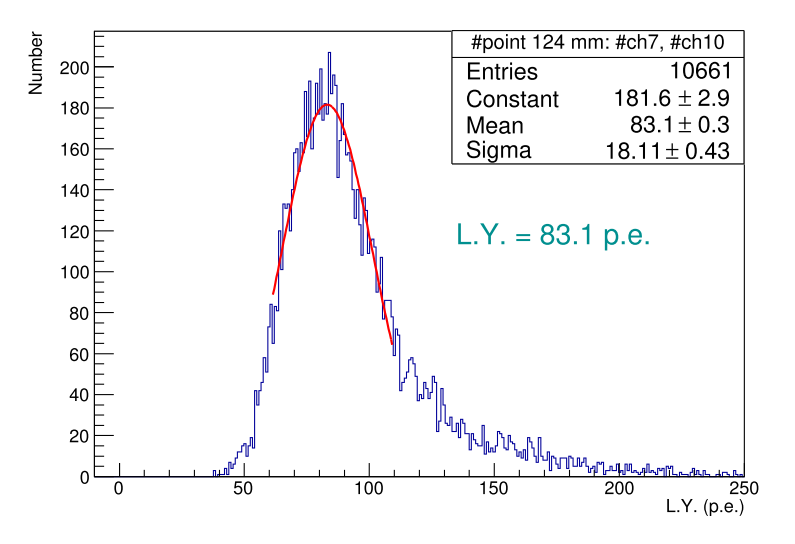
\includegraphics[width=\linewidth]{fst_light} \\ (a)
	\end{minipage}
	\begin{minipage}{0.49\linewidth}
		\centering
		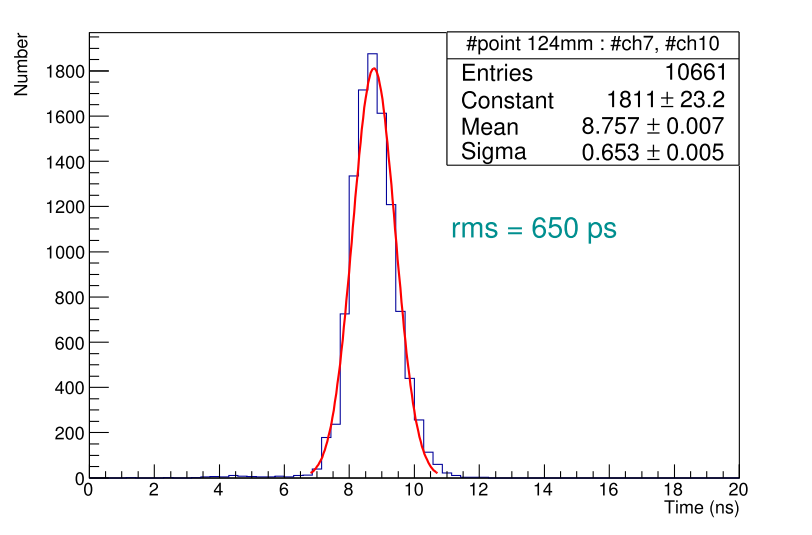
\includegraphics[width=\linewidth]{fst_time} \\ (a)
	\end{minipage}
	\caption{A light yield (a) and a time resolution (b) of the first prototype of the SuperFGD detector.}
	\label{fig:up:sfgd:1st_res}
\end{figure}

The results of the beam test were published in~\cite{Mineev2019}.

\subsection{Second CERN beamtest}
\label{sec:up:sfgd:beam2}

prototype description

electronics description

light yield
time resolution

\section{Conclusion}

% A new scintillator target is going to be built for the upgrade of the near detector. It will be placed between two HA--TPCs. The main benefits of the new target are:
% \begin{itemize}
% 	\item provide 2 tons of fiducial mass
% 	\item reconstruct muon, pion, and proton tracks with low momentum threshold
% 	\item separate electron production from photon conversion

% \end{itemize}






\chapter{Neutron tagging in SuperFGD}
\label{ch:up:neutron}
\section{Motivation}
\section{Geant4 simulation}
\section{Efficiency and energy resolution}
\section{Background estimations}
\section{Prospects for physics}
\end{document}